\documentclass[aps,prl,twocolumn,superscriptaddress,tightenlines,longbibliography, reprint]{revtex4-1}
\usepackage{graphicx, color}
\usepackage{amsmath, amssymb, amsfonts, mathrsfs, ulem}
\usepackage{times}
\usepackage[margin=1in]{geometry}

%\bibliographystyle{apsrev4-1}

\newcommand{\eg}{e.g.,}

\newcommand{\vecx}{$\vec{x}$}
\newcommand{\dt}{$\Delta$}
\newcommand{\dtR}{$\Delta_{\textrm{R}}$}
\newcommand{\R}{$\mathscr{R}$}
\newcommand{\V}{$\mathscr{V}$}
\newcommand{\SV}{$S_{\mathrm{V}}$}
\newcommand{\SR}{$S_{\mathrm{R}}$}

\newcommand{\persec}{$\textrm{s}^{-1}$}
\newcommand{\rate}{$\dot{\gamma}$ }

\begin{document}

\title{Simulating Molecular Dynamics with Large Timesteps using Recurrent Neural Networks}

\author{JCS Kadupitiya}
\email{kadu@iu.edu}
\affiliation{Intelligent Systems Engineering, Indiana University, Bloomington IN 47408, USA}
\author{Geoffrey C. Fox}
\email{gcf@iu.edu}
\affiliation{Intelligent Systems Engineering, Indiana University, Bloomington IN 47408, USA}
\author{Vikram Jadhao}
\email{vjadhao@iu.edu}
\affiliation{Intelligent Systems Engineering, Indiana University, Bloomington IN 47408, USA}

\begin{abstract}
Molecular dynamics simulations rely on numerical integrators such as Verlet to solve the Newton's equations of motion. Using a sufficiently small timestep to avoid discretization errors, Verlet integrators generate a trajectory of particle positions as solutions to the equations of motions. We introduce an integrator based on recurrent neural networks that is trained on trajectories generated using Verlet integrator and learns to propagate the dynamics of particles with timestep up to 4000 times larger compared to the Verlet timestep. We demonstrate significant net speedup of up to 32000 for few-particle (1 - 16) 3D systems and over a variety of force fields. 
\end{abstract}

\maketitle

\paragraph{Introduction}
Molecular dynamics (MD) simulations are powerful tools for investigating the microscopic origins of a wide range of material phenomena \cite{frenkel,glotzer2015assembly,brunk2019computational,beckstein2004not,qiao2004charge,hadden2018all}.
MD method solves the Newton's equation of motion for a system of many particles and presents the solution in the form of a trajectory of particles (sequence of configurations, \eg\ positions) at discrete time values. At the heart of the method is the integrator that propagates the configuration of the system one small timestep at a time. Verlet integrators are a popular choice for this operation \cite{verlet1967computer}. 
For example, the ordinary Verlet integrator:
%\vspace*{-2pt}
\begin{equation} \label{eq:ov}
    \vec{x}(t + \Delta) = 2\vec{x}(t) - \vec{x}(t-\Delta) +
\Delta^2 \frac{\vec{f}}{m} + O(\Delta^4)
%\vspace*{-2pt}
\end{equation}
updates the current position $\vec{x}(t)$ at time $t$  to the future position $\vec{x}(t + \Delta)$ after timestep \dt\ using the previous position $\vec{x}(t - \Delta)$ and the force $\vec{f}$ at time $t$ that is assumed to be an analytically known function of $\vec{x}$. Here we have adopted the notation for a single particle of mass $m$; generalization to many particles is straightforward.
With $\vec{x}(t +\Delta)$ as the current position, and $x(t)$ as the previous, the propagation is continued further. 
The term $O(\Delta t^4)$ denotes the incurred error. 

Equation \ref{eq:ov} suggests that the Verlet integrator (\V) requires a sequence of 2 position coordinates ($\vec{x}_t, \vec{x}_{t-\Delta t}$) in order to evolve the position forward by \dt\ (we will call this the Verlet timestep). However, the integrator also uses the force term $\vec{f}$ and mass $m$ to process the position update. It is possible to infer $\vec{f}$ using the information encoded in the stream of position data such that the time evolution can be done with just a sequence of positions as input.
We illustrate this with a 1-dimensional example of a particle experiencing simple harmonic motion governed by the force $f = -k x$. It can be shown that the particle position can be accurately evolved to $t+\Delta t$ via the function $\mathcal{V}\left(x_t, x_{t-\Delta t}, x_{t - 2\Delta t}\right) = x_{t-\Delta}^{-1}\left( x_{t}^2 - x_{t-\Delta}^2 + x_{t}x_{t-2\Delta} \right)$ that uses a sequence of 3 positions (the information about $f$, $m$, and \dt\ is hidden in the input sequence). 
\begin{figure}[thb]
\centering
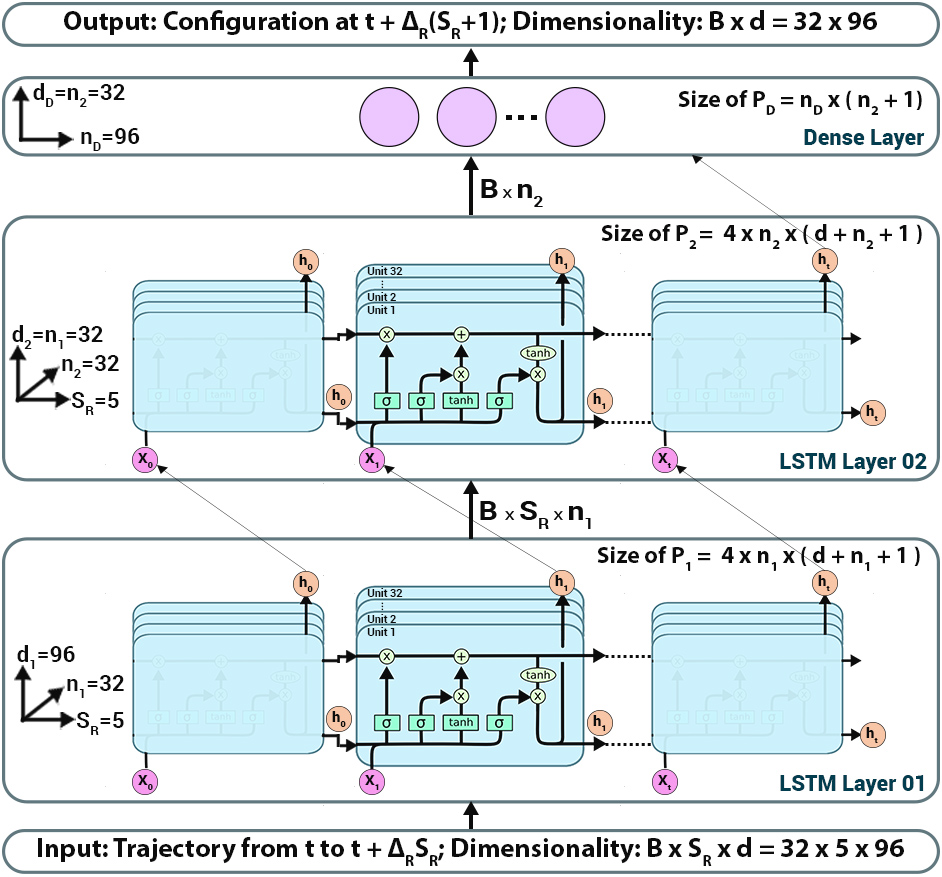
\includegraphics[width=0.48\textwidth]{figures/fig1.jpg}
%\vspace*{-20pt}
\caption{\R\ integrator based on RNN propagates the single timestep (\dtR) evolution of the $N$ particle system characterized by input features of size $d$. Input system and LSTM parameters are shown for $N=16$. Symbols are defined in the main text.}
%\vspace*{-20pt}
\label{fig:LSTMArchitecture}
\end{figure}
This idea can be extended to a general system where one could simulate the dynamics (time evolution) via the operator function $\mathcal{V}$: $\vec{x}(t+\Delta) = \mathcal{V}\left(\vec{x}_t,  \vec{x}_{t-\Delta}, \ldots \vec{x}_{t-n_V\Delta}\right)$ that takes a sequence of $n_V$ positions and propagates the particle $\Delta$ forward in time. 
However, it becomes challenging to derive $\mathcal{V}$ in a simple functional form like above for general systems with many particles, as such one defaults to Equation \ref{eq:ov} for implementing the time evolution. 
We show that deep learning can be used to derive operators like $\mathcal{V}$ for different force fields, and we demonstrate that these operators can simulate the dynamics using a timestep that is orders of magnitude larger than \dt.

The use of deep learning in sequence processing and time series prediction problems has been well studied by industry for different applications including voice recognition and translation, pattern recognition in stock market data, and ride-hailing \cite{gcfref6}. Recurrent neural networks (RNN) are established DL tools in these applications. 
\begin{figure*}[htb]
\centering
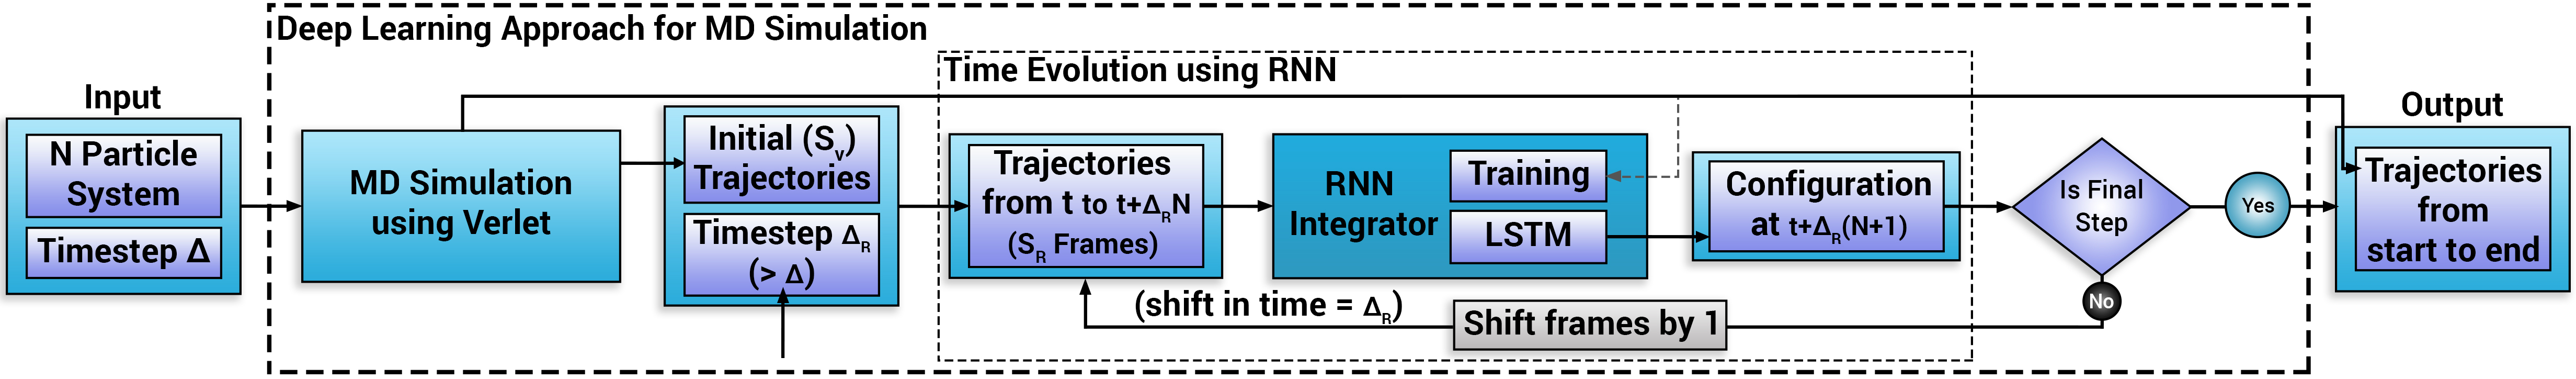
\includegraphics[width=1.0\textwidth]{figures/fig2.jpg}
%\vspace*{-20pt}
\caption{Overview of the deep learning approach based on recurrent neural networks for molecular dynamics simulations.}
%\vspace*{-15pt}
\label{fig:RNN_overview}
\end{figure*}
RNNs process input sequence data and maintain a vector $\vec{h}_t$ known as the ``hidden state'' for each recurrent cell to model the temporal behavior of sequences through directed cyclic connections between its cells. $\vec{h}_t$ is updated by applying a function $f$ to the previous hidden state ($\vec{h}_{t-1}$) and the current input ($\vec{x}_{t}$).
The cells are arranged in a fashion where they will fire when the right sequence is fed. 
A common choice for $f$ is the Long Short Term Memory networks (LSTM). 
An LSTM unit contains a cell which is the memory of the unit, and three gates (input gate, output gate, and forget gate) which regulate the flow of information into and out of the cells. This gated architecture allows the LSTM to remember longer dependencies of the sequences fed into the network and deal with the exploding and vanishing gradient problems encountered while training RNNs (see SI).

We introduce an operator $\mathscr{R}$ based on RNN derived using LSTMs (Figure \ref{fig:LSTMArchitecture}) that employs a sequence $S_R$ of current and past positions up to time $t$ to predict the future position
at time $t+$\dtR: $\vec{x}(t+\Delta_{\textrm{R}}) = \mathscr{R}\left[\vec{x}_t, \vec{x}_{t -\Delta_{\textrm{R}}}, \ldots, \vec{x}_{t - S_R\Delta_{\textrm{R}}}\right]$
where \dtR\ is the timestep associated with the RNN integrator. 
\R\ can be written as $\mathscr{R} \{x\}= \mathscr{D} [ \mathscr{L}_2 [ \mathscr{L}_1 [ \{x\} ] ] ]$,
where $\mathscr{D}$, $\mathscr{L}_1$ , $\mathscr{L}_2$ are operators associated with the dense layer, first LSTM layer, and second LSTM layer of the RNN respectively, and \{x\} is a shorthand for the sequence $\vec{x}_t, \vec{x}_{t -\Delta_{\textrm{R}}}, \ldots, \vec{x}_{t - S_R\Delta_{\textrm{R}}}$. These layers are stacked up on each other as explained in Figure \ref{fig:LSTMArchitecture} such that the output of one (\eg\ $\mathscr{L}_1$) becomes the input for another ($\mathscr{L}_2$). Each of these layer operators contains a set of parameters in the form of weights, biases, and activation functions. For example, the first hidden layer $\mathscr{L}_1$ is characterized with weights $W, U$, and bias $b$. It takes an input vector $\{x\}$ and outputs hidden state vectors $\{h\} = \mathscr{L}_1 [\{x\}, W_{1f}, U_{1f}, b_{1f}, \ldots , W_{1c}, U_{1}, b_{1c}]$.
These hidden states are fed as input to the $\mathscr{L}_2$ operator characterized with its own set of weights and biases. A similar connection is made between $\mathscr{L}_2$ and $\mathscr{D}$. Post training, these layers acquire well-determined values for all the parameters such that an integrator operator $\mathscr{R}$ emerges akin to the $\mathcal{V}$ operator in the illustrative example above, with the more explicit expression:
\begin{equation}  \label{eq:RNN_Operator2}
    \mathscr{R}[\{x\}] = \mathscr{D} [\mathscr{L}_2 [\mathscr{L}_1  [ \{x\}, \{P_1\}], \{P_2\}], \{P_D\} ],
\end{equation}
where $\{P_1\}$, $\{P_2\}$, $\{P_D\}$ are trainable parameters associated with LSTM layer 1, LSTM layer 2, and the dense layer respectively.
\R\ in Equation \ref{eq:RNN_Operator2} characterized with up to $100,000$ parameters can be considered as a reformulation of the ordinary Verlet integrator \V\ (Equation \ref{eq:ov}). This computational complexity accounts for its ability to handle much larger timesteps in driving MD simulations as we demonstrate below.
Note that while, for the ease of exposition, we showed how RNNs can describe the ordinary Verlet integrator, the derivation can be readily adapted to describe the velocity Verlet integrator (see SI). In what follows, \V\ denotes the velocity Verlet integrator.

\begin{figure*}[htb]
\centering
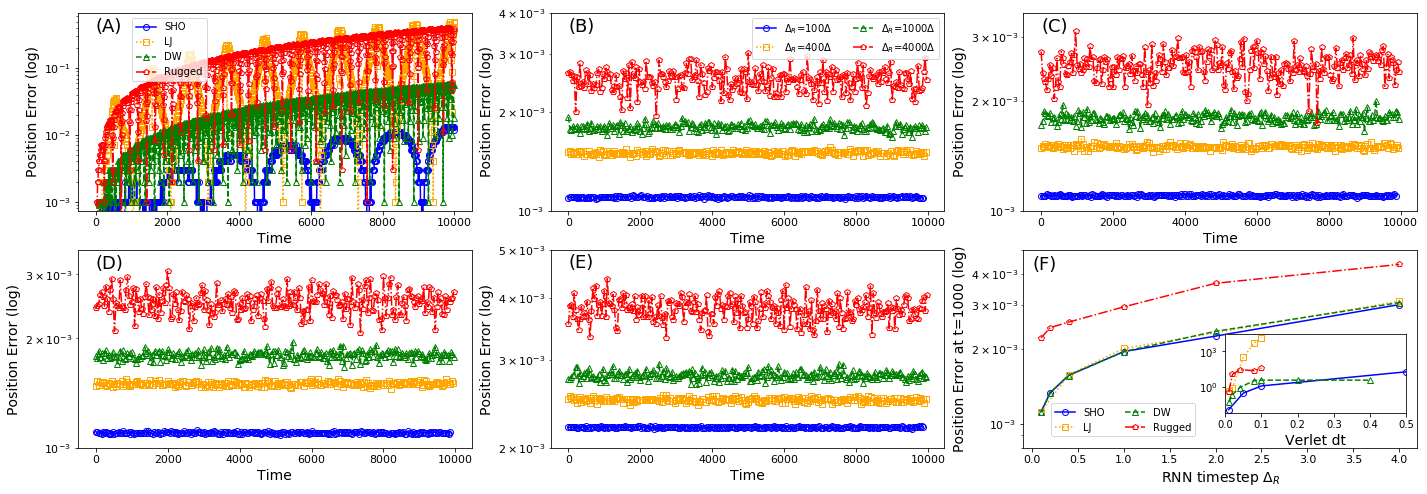
\includegraphics[width=1.0\textwidth]{figures/fig3.png}
%\vspace*{-20pt}
\caption{Errors (log scale) in position updates (trajectory) for 1D simulations. Results are shown for 4 potentials: SHO with $m=10$, $k=1$, LJ with $m=1$, $x_0=2$, DW with $m=1$, $x_0=-2$ and rugged with $m=1$, $x_0=-6$. Results are compared to respective ground truth results obtained using \V\ with $\Delta = 0.001$. (A) Errors using \V\ with  timestep $dt = 10\Delta$. (B), (C), (D), and (E) show trajectory errors using \R\ for SHO, LJ, DW, and rugged potentials respectively for $\Delta_R = 100\Delta$ (circles), $400\Delta$ (squares), $1000\Delta$ (triangles), and $4000\Delta$ (pentagons).  (F) Error incurred in position updates using \R\ at $t=1000$ vs. timestep \dtR\ for the 4 potentials; inset shows corresponding error using \V\ vs. Verlet timestep $dt$.}
%\vspace*{-15pt}
\label{fig:manypotentials}
\end{figure*}

\paragraph{Related Work}
The key related work focuses on DL to learn differential equations and replicate numerical integrators \cite{raissi2018hidden, raissi2018multistep, long2017pde, chen2018neural, endo2018multi, breen2019newton, chen2019symplectic, tronarp2020bayesian}. Generally, these integrators have been derived to operate with the time discretization associated with the baseline integrator timestep $dt$. Their applications have been demonstrated on relatively simple 1D systems governed by ordinary differential equations. Few studies have probed the DL applications to learn partial differential equations \cite{long2017pde}.
Research more closely related to ours includes recent approaches to improve the accuracy of integrators at a higher $dt$ \cite{shen2020deep,raissi2018multistep}. 
Shen et. al \cite{shen2020deep} have developed an artificial neural network (ANN) based Euler method for numerical integration with high $dt$ by approximating the local truncation error with deep neural networks to obtain accurate solutions with $dt$ up to 200 times larger than the baseline Euler approach. As applications, they have shown the approach to work on 1D systems and relatively simple 2-body problems. For the 1D problems, a 100 fold increase in the timestep (from 2$\times$ to 200$\times$) led to an increase in the prediction error by over 3 orders of magnitude. %603673.5\%. 
In this paper, we show that RNN-based integrators can limit the rise in the error with increasing timestep ($>1000\times$ the baseline) to within an order of magnitude, even for the complex 3D systems.

Instead of explicit time evolution of the system with an operator that emulates the numerical time integration, other related work has focused on using DL to learn the Hamiltonian of simple physical systems and respect conservation laws in an unsupervised manner  \cite{greydanus2019hamiltonian,cranmer2020lagrangian,chen2019symplectic,battaglia2016interaction, chang2016compositional, rupp2012fast, chmiela2017machine,sanchez2019hamiltonian, shin2020convergence}.
Here, neural networks observe the positions and momenta (input) and produce the Hamiltonian as output, in some cases leveraging the information that the partial derivatives of the output with respect to inputs are the time derivatives of the inputs \cite{greydanus2019hamiltonian}.
Hamiltonian neural networks \cite{greydanus2019hamiltonian}, Lagrangian neural networks \cite{cranmer2020lagrangian}, and symplectic RNNs \cite{chen2019symplectic} are examples of these DL approaches that have been shown to learn the physics of simple systems such as spring-mass problems in 1D. 

In materials science and engineering research, recent years have seen a surge in the use of machine learning (ML) to enhance the performance of simulations and analyze the data they generate  \cite{ferguson2017machine,mehta2019high,butler2018machine,gcfref1,gcfref3,sam2017,melko2017,glotzer2017,wang2017mesoscale,fu2017,guo2018adaptive,botu2015adaptive,kadupitiya2020ml,kadupitiya2020ml,long2015machine,moradzadeh2019molecular}. However, to the best of our knowledge, DL-based advancements at the level of re-formulating the integrator driving the MD simulation have not been made. Generally, ML applications in MD simulations of materials have centered on accelerating the sampling of systems with rugged free-energy landscapes \cite{guo2018adaptive}, generating new configuration updates in latent-space (low-dimensional) variables in ab initio MD simulations of nuclei-electron systems \cite{botu2015adaptive}, auto-tuning timestep in MD simulations of ions near nanomembranes \cite{kadupitiya2020ml}, and classifying assembly landscapes employing MD-generated particle trajectories \cite{long2015machine}. Furthermore, DL has been used to derive networks that produce ``surrogates'' of large-scale simulations, including MD simulations \cite{aspuru2019,kadupitiya2019machine,moradzadeh2019molecular, kadupitiya2020machine,kasim2020up}. 

We build on these recent works with the goal towards enabling simulations of complex 3D systems of particles interacting with commonly employed potentials describing soft-matter systems (\eg\ Lennard-Jones potential),  and develop a DL approach that learns the Hamiltonian of the system and the underlying differential equation from the high-dimensional configuration space (trajectories) to perform the time evolution with large timesteps.  
We show that RNN with generic LSTM models, with minimal architectural changes, can learn both the dynamical equations and the interaction potentials driving the dynamics of particles. 
Most importantly, we demonstrate that our integrator performs accurate time evolution of 1D systems and complex 3D systems with realistic boundary conditions and over a variety of force fields using large timesteps (up to $4000\times$ the baseline). To the best of our knowledge, in terms of number of particles, timesteps for trajectory evolution, and the complexity of the systems probed, our approach fares better than existing ones in metrics such as trajectory errors, energy conservation tracking, and net speedup.

\paragraph{Methods}
Figure \ref{fig:RNN_overview} describes the DL approach using \R\ to evolve the dynamics of an $N$ particle system with timestep \dtR. 
\R\ is trained using particle trajectories generated via \V\ with small \dt $=0.001 <$ \dtR\ such that the Verlet result can be considered as the ground truth. 
Input system attributes and $\Delta$ are fed to \V\ to simulate the dynamics and obtain $S_{\mathrm{V}} = \Delta_{\mathrm{R}}(S_R - 1)/\Delta$ number of configurations. Out of \SV, \SR\ number of configurations (frames) separated by \dtR\ are distilled to feed the \R\ operator (\SR\ is the sequence length). \R\ predicts the time evolution of the system after \dtR. Until the end of the simulation, the input sequence to \R\ is left shifted to discard the oldest time frame, and the latest frame predicted by \R\ is appended to the right of the sequence. The adjusted input sequence is fed to \R\ to evolve the system \dtR\ further in time. 

\begin{figure*}[hbt]
\centering
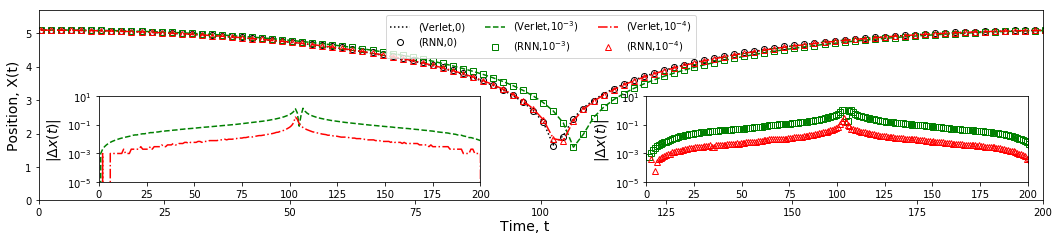
\includegraphics[width=1.0\textwidth]{figures/fig4.png}
%\vspace*{-20pt}
\caption{Lyapunov instability tests in 1D simulations of a particle in an LJ potential with $m=1, x_0=5.1$ using \V\ with \dt $=0.001$ and \R\ with $\Delta_{\mathrm{R}}=0.1 = 100$\dt. Legend indicates (integrator, $\delta p$) where $\delta p$ represents the small momentum shift introduced at the start of trajectory. Lines and markers are the results of simulations driven by \V\ and \R\ integrators respectively. Outset shows the trajectory for $\delta p = 0, 10^{-3}, 10^{-4}$. Left and right insets show the absolute difference between trajectories with $\delta p \ne 0$ and $\delta p = 0$ ($\Delta x(t)$=$|x(t,0)-x(t,\delta p)|$) as produced by \V\ and \R\ respectively.
}
%\vspace*{-15pt}
\label{fig:lyapunov}
\end{figure*}

The training and testing datasets are generated and processed for $N \in (1,16)$ by changing the parameters characterizing the potential energies and the physical attributes describing the particles. Four different potentials are considered: 1) simple harmonic oscillator (SHO), 2) Lennard-Jones (LJ), 3) double well (DW), and 4) rugged (see SI). 
In these initial studies, we select  datasets generated by sweeping parameters that mainly shift the initial configuration (\eg\ $x_0$ in LJ) or scale the particle attributes (\eg\ mass $m$ in LJ), and in some cases change the shape of the potential energy (\eg\ $k$ in SHO).
\R\ integrator with  LSTM layer 1, LSTM layer 2, and final dense layer (Figure \ref{fig:LSTMArchitecture}) is implemented in TensorFlow for regression of the particle trajectories using $n_1$, $n_2$, and $n_D$ number of hidden units respectively (specific values depend on the system). 
\R\ takes a $B \times$ \SR $\times d$ dimensional vector as input where $B$ and $d$ refer to batch and feature size respectively.
All the parameters $\{P\}$ (weights, biases) describing the layers are trained with an error backpropagation algorithm, implemented via a stochastic gradient descent. 
Data preparation and preprocessing, feature extraction, and LSTM implementation details are provided in the SI. 

\paragraph{Experiments and Empirical Results}

We now compare the empirical results (\eg\ trajectories, energies) obtained from simulations using \R\ against the baseline velocity Verlet integrator \V. 
%\paragraph{1D simulations}
Our first experiments are on testing \R\ to predict the time evolution of single particle systems in 1D. Training datasets of trajectories simulated using \V\ with \dt$=0.001$ up to $t=200$ are used.
We find that the errors in positions (trajectory errors) predicted by \R\ do not increase over time for $t$ up to 10000, and are $O( 10^{-3})$ for all systems studied with $\Delta_{\textrm{R}} \in (100\Delta,4000\Delta)$ (Figure \ref{fig:manypotentials} B, C, D, E). The errors rise with increase in \dtR\ and the complexity of the potential (\eg\ higher for rugged than LJ) but remain within an order of magnitude (Figure \ref{fig:manypotentials} F). 
The average error values across different potentials for \dtR\ $= [100\Delta, 400\Delta, 1000\Delta, 4000\Delta]$ are $\approx 0.001, 0.002, 0.003, 0.004$ respectively.
On the other hand, the trajectory errors incurred using \V\ with timestep 10\dt\ show exponential increase with $t$ and with rising timestep for all potentials considered (Figure \ref{fig:manypotentials} A and F). 
Similarly, velocity $v$ and position $x$ predictions produced by \R\ exhibit small trajectory errors, and the phase diagram ($v$ vs. $x$) and the total energy track the ground truth associated with the respective potential energy (\eg\ LJ or SHO) for $t$ up to 10000 and \dtR\ up to 4000\dt\ (SI Figure \ref{fig:phasespace}). \R\ learns the energy conservation feature associated with the dynamics of these systems obeying Newton's equations of motion.

Next set of experiments involve assessing the stability of the solutions (trajectories) predicted by the integrator \R. 
This is typically discussed in terms of Lyapunov instability (LI) which states that close-by trajectories diverge exponentially \cite{posch1988lyapunov, venneri1987simple}. LI is present in standard Verlet integrators for many potentials.
Trajectories of a particle of $m=1$ in 1D LJ potential generated using \V\ are used for these experiments. 
A small perturbation in the momentum $\delta p$ is introduced at the start to investigate its effects on long-time evolution of the trajectory.
We find that the RNN surrogate inherits the characteristic LI of \V\ (Figure \ref{fig:lyapunov}). 
As $\delta p$ increased from $10^{-4}$ to $10^{-3}$, the trajectories predicted by \R\ (\V) exhibit similar average divergences from $0.0153$ ($0.0152$) to $0.149$ ($0.148$). 

Our final set of experiments probe the extension of the proposed DL approach to $N>1$ particles. $N=3,8,16$ particle systems with LJ interaction potential are used. \R\ is trained to learn from trajectories generated using \V\ ($\Delta=0.001$) in a cubic box with periodic boundary conditions (PBC) or in a spherical hard-wall confinement with reflective boundaries. 
We find that \R\ successfully evolved the positions and velocities of particles up to time $t = 1$ million for all the $N$-particle systems studied with \dtR\ up to 4000\dt.
In the interest of brevity, we only discuss the results of experiments on the $N=16$ system in PBC. The training dataset size for this study involved
dynamics up to $t=2000$. The random initial configuration for testing \R\ was selected outside the training dataset.
We find that the trajectory error (computed as an average over 16 particles) associated with the positions predicted by \R\ for \dtR$=100$\dt\ to $4000$\dt\ is $O(10^{-3})$ for all times (SI Figure \ref{fig:manyparticleSI}), exhibiting a behavior similar to the 1D results (Figure \ref{fig:manypotentials}).
The total energy $E_t \equiv E(t)$ and the energy deviation $\delta E(t) = (E_t-E_0)/E_0$ of the system, extracted from the predicted position and velocity data, show that \R\ conserves the total energy of the system ($\delta E(t)$ $\lesssim 10^{-3}$) for up to $t=10^6$, closely tracking the ground truth results for all \dtR\ (from 100\dt\ to 4000\dt). In strike contrast, the baseline \V\ integrator suffers from growing accumulated error of $>10^{-1}$ when simulated with timestep of 40\dt\ and exhibits a rapid divergence in the energy for $t>10^5$ (with associated average trajectory error of $10^9$ at $t\approx10^5$; SI Figure \ref{fig:manyparticleSI}).

\begin{figure}[htb]
\centering
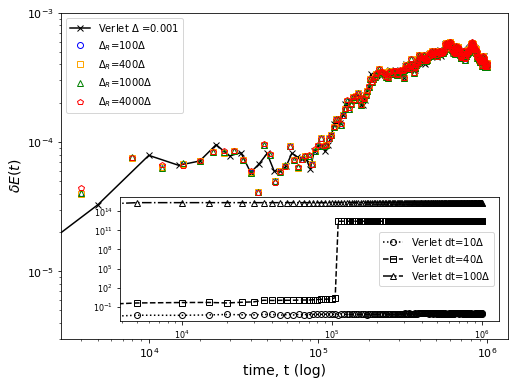
\includegraphics[width=0.48\textwidth]{figures/fig5.png}
%\vspace*{-20pt}
\caption{Energy conservation using \R\ in a $N=16$ particle 3D simulation with LJ interactions ($\epsilon=2$ and $m=1$) in PBC with initial positions randomly selected and initial velocities set to 0. Black lines are the ground truth results obtained using \V\ with $\Delta=0.001$. Outset shows the energy deviation $\delta E$ (log scale) vs. time $t$ (log scale) predicted by \R\ for \dtR = 100\dt, 400\dt, 1000\dt, 4000\dt. Inset shows the same for time evolution using \V\ with timestep 10\dt, 40\dt, and 100\dt. Note the order of magnitude difference between the outset and inset y-axis values. 
}
%\vspace*{-15pt}
\label{fig:manyparticle}
\end{figure}

\paragraph{Speedup}

The DL approach uses Verlet integrator to kickstart the MD simulation and \R\ to evolve the dynamics forward in time. The calculation of net speedup $S_p$ should incorporate this detail. Without accounting for the time spent on creating training datasets (total $<24$ hours for the experiments shown), $S_p$ can be defined as:
\begin{equation}\label{eq:speedup}
    S_p = t_{\mathrm{V}}S_{\mathrm{T}}/
    \left[S_{\mathrm{V}} t_{\mathrm{V}} + \left(S_{\mathrm{T}} - S_{\mathrm{V}}\right) t_{\mathrm{R}} \Delta / \Delta_{\mathrm{R}}\right]
\end{equation}
where $S_{\mathrm{T}}$ is the total number of steps needed if the time evolution is performed only using \V, $t_{\mathrm{V}}$ is the time for one forward step propagation using \V, and
$t_{\mathrm{R}}$ is the time for one forward step propagation using \R\ (other symbols are defined above).
$S_p$ is 1 if \SR$=0$ (no time evolution using \R). As most MD simulations are expected to run for long times, in the limit $S_{\mathrm{T}} \gg S_{\mathrm{V}}$, we obtain $S_p \approx t_{\mathrm{V}}\Delta_{\mathrm{R}} / (t_{\mathrm{R}}\Delta)$.
For example, for the system of 16 LJ particles with  $t_{\mathrm{v}}\approx 0.04392$ seconds, $\Delta =0.001$, $t_{\mathrm{R}} \approx 0.0026$ seconds, and $\Delta_{\mathrm{R}}=4.0$, we find $S_p > 10^4$. Table \ref{tab.ml.speedups} shows $S_p$ obtained in different experiments for different \dtR.  
For time evolution up to $t=10^6$ requiring $S_T=10^9$ steps, we find $S_p$ up to $45\times$ for 1D systems, and from $230\times$ to $32000\times$ for the many particle simulations with LJ interaction potential.
$S_p < 1$ data is generally for experiments with 1D systems for $\Delta_{\mathrm{R}} = 100$\dt, $200$\dt\ and when $t_{\mathrm{V}} < t_{\mathrm{R}}$ (that is, for the 1D cases where the computational cost for time evolution using \V\ is smaller than that for \R).
\begin{table}[htbp]
%\vspace*{-15pt}
\caption{Net Speedup $S_p$ of the DL approach}
%\vspace*{-10pt}
\begin{center}
\begin{tabular}{|c|c|c|c|c|c|c|}
\hline
\textbf{Expt. / \dtR} & \textbf{0.1} & \textbf{0.2} & \textbf{0.4} & \textbf{1.0} & \textbf{2.0} & \textbf{4.0} \\
\hline
\textbf{SHO} & 0.5 & 1.3 & 3.2 & 8.6 & 20.0 & 45.0 \\
\hline
\textbf{LJ} & 0.9 & 1.5 & 3.9 & 12.8 & 22.5 & 42.3 \\
\hline
\textbf{Double-well} & 0.6 & 1.2 & 2.8 & 8.7 & 17.3 & 38.0 \\
\hline
\textbf{Rugged} & 0.4 & 0.8 & 2.1 & 4.7 & 9.7 & 20.6 \\
\hline
\textbf{LJ, 8} & 600 & 1000 & 1500 & 5500 & 8300 & 12000 \\
\hline
\textbf{LJ, 16} & 3000 & 4900 & 7100 & 20000 & 28000 & 32000 \\
\hline
\end{tabular}
\label{tab.ml.speedups}
\end{center}
%\vspace*{-15pt}
\end{table}
\paragraph{Conclusion}
We introduced an integrator based on recurrent neural networks which can learn the dynamics of many particle systems described by the Newton's equations of motion using trajectory data generated via the traditional Verlet integrators. 
To evaluate our integrator, we showed that it exhibits excellent energy conservation and produces accurate predictions of the trajectories of systems with up to 16 particles using up to $4000 \times$ larger timestep than the Verlet integrators.
We also showed that our integrator inherits the Lyapunov instabilities of the Verlet integrator. Finally, we demonstrated significant net speedup over a variety of interaction potentials and total number of particles.
Future work will aim to generalize this approach to make it applicable to systems with large number of particles in part by the use of alternative deep learning approaches including non-recurrent networks such as transformers \cite{gcfref7}.

\subsection{Acknowledgments}
This work is partially supported by the National Science Foundation (NSF) through awards 1720625 and DMR-1753182. G.C.F was partially supported by NSF CIF21 DIBBS 1443054 and CINES 1835598 awards.
Simulations were performed using the Big Red III supercomputing system.

%\mbox{~}
%\clearpage
\section{Supporting Information}\label{integrators}

\subsection{Numerical Integration}
In MD simulations, one needs to follow the motion of $N$ particles interacting with potential energy $U$. Using $U$, the forces on particles can be derived via $\vec{F} = - \vec{\nabla}U$, and the motion of particles gets determined via Newton's equation $\vec{F} = - m\vec{a}$ ($\vec{\nabla}$ is the gradient operator). There are many numerical integration methods that can integrate these equations. Among these, the velocity Verlet integrator is a very popular choice and we have used this integrator to generate the ground truth for the experiments described in this paper. The velocity Verlet integrator \V\ is given by the following equations:
\begin{equation} \label{eq:vv1}
    \vec{x}(t + \Delta) = \vec{x}(t) + \Delta \vec{v}(t) +
\frac{\Delta^2}{2m} \vec{f}(t),
\end{equation}
\begin{equation} \label{eq:vv2}
    \vec{v}(t + \Delta) = \vec{v}(t) + \frac{\Delta}{2m} \left(\vec{f}(t)+\vec{f}(t+\Delta )\right).
\end{equation}
\V\ updates the current position $\vec{x}(t)$ at time $t$  to the future position $\vec{x}(t + \Delta)$ after timestep \dt\ using the current velocity $\vec{v}(t)$ and the force $\vec{f}$ at time $t$. Here we have adopted the notation for a single particle of mass $m$; generalization to many particles is straightforward. Similarly, the integrator updates the current velocity $\vec{v}(t)$ at time $t$  to the future velocity $\vec{v}(t + \Delta)$ after timestep \dt\ using the force $\vec{f}$ at time $t$ and the force $\vec{f} (t+ \Delta)$ at time $t+\Delta$. Note that after the position update in Equation \ref{eq:vv1}, the forces will need to be re-evaluated to update the velocities in Equation \ref{eq:vv2}. With $\vec{x}(t +\Delta)$ as the current position and $\vec{v}(t +\Delta)$ as the current velocity, the propagation is continued further. 

Equations \ref{eq:vv1} and \ref{eq:vv2} suggest that the velocity Verlet integrator requires the current position ($\vec{x}_t$) and velocity coordinates ($\vec{v}_t$) in order to evolve the dynamics forward by $\Delta$. Further, the integrator also uses the force term $\vec{f}$ and mass $m$ to process the update. It is possible to infer $\vec{f}$ using the information encoded in the stream of position data and velocity data such that the time evolution can be done with just a sequence of positions and velocities as input. Similar to ordinary verlet, we illustrate this with a 1-dimensional example of a particle experiencing simple harmonic motion governed by the force $f = -k \vec{x}$. It can be shown that 
the particle position can be accurately evolved to $t+\Delta t$ via the function $x_{t-\Delta}^{-1}\left( x_{t}^2 - \Delta (x_{t-\Delta} v_{t} + x_{t-\Delta} v_{t}) \right)$ that uses a sequence of 2 positions, 2 velocities and $\Delta$ (the information about $f$ and $m$ is hidden in the input sequence). Similarly, It can be shown that 
the particle velocity can be accurately evolved to $t+\Delta t$ via the function $(x_{t-\Delta}+ x_{t})^{-1}\left( (x_{t-\Delta}+ x_{t})v_t + (v_{t} - v_{t-\Delta})(x_{t} + x_{t+\Delta}) ) \right)$ that uses a sequence of 3 positions and 2 velocities. This idea can be extended to a general system where one could simulate the dynamics (time evolution) via the operator function $\mathcal{V}$: $\vec{x}(t+\Delta), \vec{v}(t+\Delta) = \mathcal{V}\left(\vec{x}_t,  \vec{x}_{t-\Delta}, \ldots \vec{x}_{t-n_V\Delta}, \vec{v}_t,  \vec{v}_{t-\Delta}, \ldots \vec{v}_{t-k_V\Delta}, \Delta \right)$ that takes a sequence of $n_V$ positions, $k_V$ velocities, and $\Delta$ to propagate the particles $\Delta$ forward in time.

\subsection{LSTM Networks}
There are several architectures of LSTM units. A common architecture is composed of a cell (the memory part of the LSTM unit) and three ``regulators'', usually called gates, that regulate the flow of information inside the LSTM unit. An input gate ($i_t$) controls how much new information is added from the present input ($x_t$) and past hidden state ($h_{t-1}$) to our present cell state ($c_{t}$). A forget gate ($f_t$) decides what is removed or retained and carried forward to the current cell state ($c_{t}$) from the previous cell state ($c_{t-1}$). An output gate ($o_t$) decides what to output as the current hidden state ($h_t$) from the current cell state ($c_{t}$).
The math formulation of LSTM is given as:
\begin{align} 
f_t &=\sigma_g (W_f x_t + U_f h_{t-1} + b_f) \nonumber \\ 
i_t &=\sigma_g (W_i x_t + U_i h_{t-1} + b_i) \nonumber \\
o_t &=\sigma_g (W_o x_t + U_o h_{t-1} + b_o) \nonumber\\
\tilde{c_t} &=\sigma_h (W_c x_t + U_c h_{t-1} + b_c) \nonumber \\
c_t &= f_t \circ c_{t-1} + i_t \circ \tilde{c_t} \nonumber \\
h_t &= o_t \circ \sigma_h(c_t).
\end{align}
Here, $x_t \in \mathbf{R^d}$ is the input vector to the LSTM unit, $f_t \in \mathbf{R^h}$ is the forget gate's activation vector, $i_t \in \mathbf{R^h}$ is the input gate's activation vector, $o_t \in \mathbf{R^h}$ is the output gate's activation vector, $h_t \in \mathbf{R^h}$ is the hidden state vector also known as the output vector of the LSTM unit, $c_t \in \mathbf{R^h}$ is the cell state vector, and $\circ$ is the Hadamard  product operator.  $W \in \mathbf{R^{hxd}}$, $U \in \mathbf{R^{hxh}}$ and $b \in \mathbf{R^h}$ are the weight matrices and bias vector parameters which need to be learned during training. $\sigma_g$ and $\sigma_h$ represent sigmoid function and hyperbolic tangent functions respectively. The superscripts $d$ and $h$ refer to the number of input features and the number of hidden units respectively.

\subsection{Data Generation, Preparation, and Preprocessing}

Prior domain experience and backward elimination using the adjusted R squared is used for selecting the  significant input parameters for creating the training data set. 
This process determines which inputs are important to change the desired output. The process begins with all possible inputs and eliminates them one by one, monitoring the adjusted R squared value to determine which are important. Dropping of an input that produces a sharp spike in the R squared value is indicative of the high importance of the input parameter. 
This process is used to select the inputs parameters for the datasets described under this section. 
Unlike traditional deep neural networks where you would map the physical inputs to outputs generally distinct from inputs, the inputs and outputs for the RNN approach (integrator $\mathscr{R}$) are both trajectory data as shown in Figure \ref{fig:dataprocessing}. Traditional MD simulation ran with the velocity Verlet algorithm will have multi feature time series data (\eg\ position, velocity vectors) separated by $\Delta =0.001$ in time. To train the integrator $\mathscr{R}$, we prepare the inputs and target data as explained in Figure \ref{fig:dataprocessing}. 
\begin{figure}[htb]
\centering
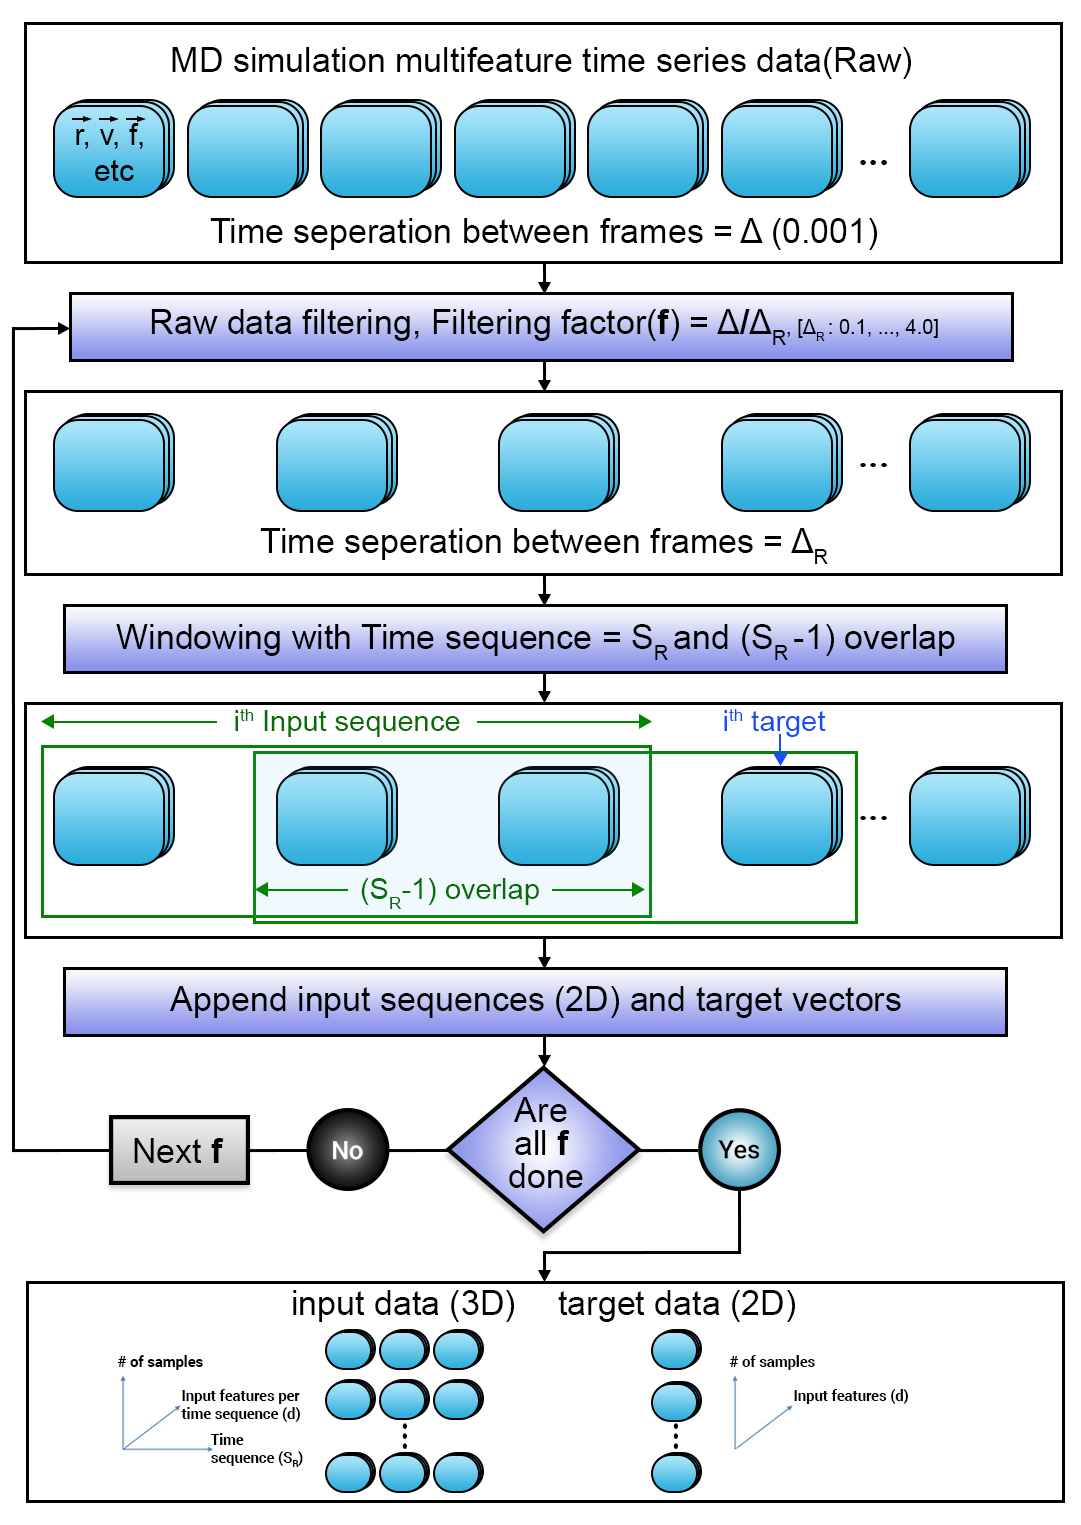
\includegraphics[width=0.48\textwidth]{figures/fig6.jpg}
%\vspace*{-20pt}
\caption{Data processing for training and testing of integrator $\mathscr{R}$}
%\vspace*{-15pt}
\label{fig:dataprocessing}
\end{figure}
Since integrator $\mathscr{R}$ will operate with different timestep $\Delta_{R}$ (\eg\ $100\Delta, 1000\Delta$), we filter the time series data with a filtering factor defined as $\Delta_{\mathrm{R}}/\Delta$ to make the data separated with $\Delta_{\mathrm{R}}$. Next, we do windowing through the time series data with the window length of $S_R$ (the RNN model sequence length), and frame overlap of $S_R -1$
to generate a sequence of length $S_R$ as input and the future configuration as the output (target). We do this repeatedly until the time series is ended and then move to the next choice for $\Delta_{R}$ and a new associated filtering factor. We do the same process for all simulation data and append all the input sequences and target vectors as shown in Figure \ref{fig:dataprocessing}. In the end, all the input sequences are expected to form a 3D matrix (number of samples $\times$ feature size ($d$) $\times$ $S_R$) and the associated output vectors form a 2D matrix (number of samples $\times$ $d$). A min-max normalization filter is applied to normalize the input data and randomly shuffle them (along the axis of the number of samples) to generate the data for training and testing $\mathscr{R}$. The entire data set is separated into training and testing sets using a ratio of 0.8:0.2.

\begin{figure}[thb]
\centering
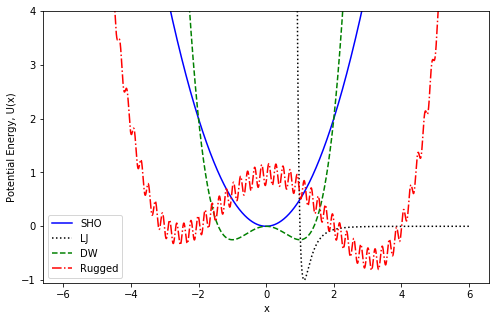
\includegraphics[width=0.48\textwidth]{figures/fig7.png}
%\vspace*{-20pt}
\caption{Potential energies associated with the 1D experiments. Solid, dotted, dashed, and dash-dotted lines represent SHO, LJ, double well, and rugged potential respectively.}
%\vspace*{-15pt}
\label{fig:potential_plots}
\end{figure}
We now describe the datasets associated with systems characterized by different interaction potential energies and physical attributes used in the experiments for training and testing \R. The potential energy functions are shown in Figure \ref{fig:potential_plots}.
For the 1D systems, the timestep (for velocity Verlet integrator) and the total time were chosen to be $\Delta = 0.001$ and $t_f = 100$.
For the 3D many particle systems, $\Delta = 0.001$ and $t_f = 2000$.
%
\paragraph{Simple harmonic oscillator (SHO)}
For this system, the potential energy is given by
\begin{equation} \label{eq:data1}
U = \frac{1}{2} k x^2,
\end{equation}
and the associated force is
\begin{equation} \label{eq:data2}
F = - k x.
\end{equation}
The dataset is generated by varying three input parameters: mass of the particle $m \in [1, 10]$, spring constant $k \in [1, 10]$, and initial position of the particle  $x_0 \in [-10, -1]$. The parameter sweep generated a data set of 500 simulations, each having 50,000 position and velocity values.

\paragraph{1D Lennard-Jones (LJ) system}
For this system, the potential energy is given by
\begin{equation} \label{eq:data5}
U(x) = 4\epsilon \left(\left(\frac{\sigma}{x}\right)^{12} - \left(\frac{\sigma}{x}\right)^{6}\right),
\end{equation}
and the associated force is
\begin{equation} \label{eq:data6}
F =  \frac{48 \epsilon}{x} \left(\left(\frac{\sigma}{x}\right)^{12} - 0.5 \left(\frac{\sigma}{x}\right)^6 \right) .
\end{equation}
The dataset is generated by varying two input parameters: mass of the particle $m \in [1, 10]$ and the initial position of the particle  $x_0 \in [1.0, 3.0]$. The parameter sweep generated a data set of 500 simulations, each having 50,000 position and velocity values.
\paragraph{Particle in a double well (DW)}
For this system, the potential energy is given by
\begin{equation} \label{eq:data7}
U = \frac{1}{4}x^4 - \frac{1}{2}x^2,
\end{equation}
and the associated force is
\begin{equation} \label{eq:data8}
F = x - x^3.
\end{equation}
The dataset is generated by varying two input parameters: mass of the particle $m\in[1,10]$ and the initial position of the particle $x_0 \in [-3.1, 3.1]$. The parameter sweep generated a data set of 500 simulations, each having 50,000 position and velocity values.
\paragraph{Particle in a rugged potential}
For this system, the potential energy is given by
\begin{equation} \label{eq:data9}
U(x) = \frac{x^4 - x^3 - 16x^2 + 4x + 48}{50}
+ \frac{\sin{(30(x+5))}}{5},
\end{equation}
and the associated force is
\begin{equation} \label{eq:data10}
F = \frac{-4x^3 + 3x^2 + 32x - 4}{50} -6 \cos{(30(x+5))}.
\end{equation}
The dataset is generated by varying two input parameters: mass of the particle $m \in [1,10]$ and the initial position of the particle  $x_0\in [-6.1,6.1]$. The parameter sweep generated a data set of 640 simulations, each having 64,000 position and velocity values.
\paragraph{Many particles interacting with LJ potential}
For this 3D system, the interaction potential energy between any two particles is given by the LJ potential:
\begin{equation} \label{eq:data11}
U(r) = 4\epsilon \left(\left(\frac{\sigma}{r}\right)^{12} - \left(\frac{\sigma}{r}\right)^{6}\right),
\end{equation}
and the associated force is
\begin{equation} \label{eq:data12}
\vec{F} =  \frac{48 \epsilon} {r^2} \left(\left(\frac{\sigma}{r}\right)^{12} - 0.5 \left(\frac{\sigma}{r}\right)^6 \right) \vec{r}.
\end{equation}
We prepared two different types of simulation boxes to generate the datasets: cubic box with periodic boundary conditions (PBC) and spherical box with reflective boundary. In each box, we performed simulations with $N=3, 8$ and $16$ particles. Each of these simulations were created as a separated dataset that yielded 6 different datasets to train and test \R. The dataset is generated by varying two input parameters: mass of the particle $m \in [1, 10]$ and the initial position of the particles  $(x_0, y_0, z_0)$ with each Cartesian coordinate chosen between $-3.0$ and $3.0$. Initial velocities were chosen to be zero. The parameter sweep generated a dataset of 5000 simulations for each of the aforementioned cases (or 30,000 simulations in total). 

\subsection{Feature Extraction and Regression}
In the interest of brevity, we only present the details of feature extraction and regression associated with the integrator $\mathscr{R}$ implemented for the most complex case of 16 particles interacting with LJ potential in 3D with PBC. An RNN with two LSTM layers and a dense layer (Figure \ref{fig:LSTMArchitecture}) is implemented in TensorFlow for regression of the prediction for the trajectories of 16 particles (position and velocity vectors). Outputs of the LSTM layers are wrapped with the $\tanh$ function. No wrapping functions are used in the final dense layer of the model as integrator $\mathscr{R}$ was trained for regression. The weights and biases of all the layers are trained with an error backpropagation algorithm, implemented via a stochastic gradient descent procedure. 
The size of the hidden layers was chosen depending on the model complexity and data dimensions. By performing a grid search, hyper-parameters such as the number of units per each of the two layers ($n_1$, $n_2$) and final dense layer ($n_D$), batch size ($B$), and the number of epochs are optimized to 32, 32, 96, 256, and 2500 respectively. 
Here we have not done a thorough hyper-parameter optimization but have identified reasonable values for key choices -- the architecture and the size of the network, and the length of time series.
\R\ takes a $B \times$ \SR $\times d$ dimensional vector as input, where $B$ and $d$ refer to batch and feature size respectively. For the 3D system considered above, $d=96$.

\begin{figure*}[htb]
\centering
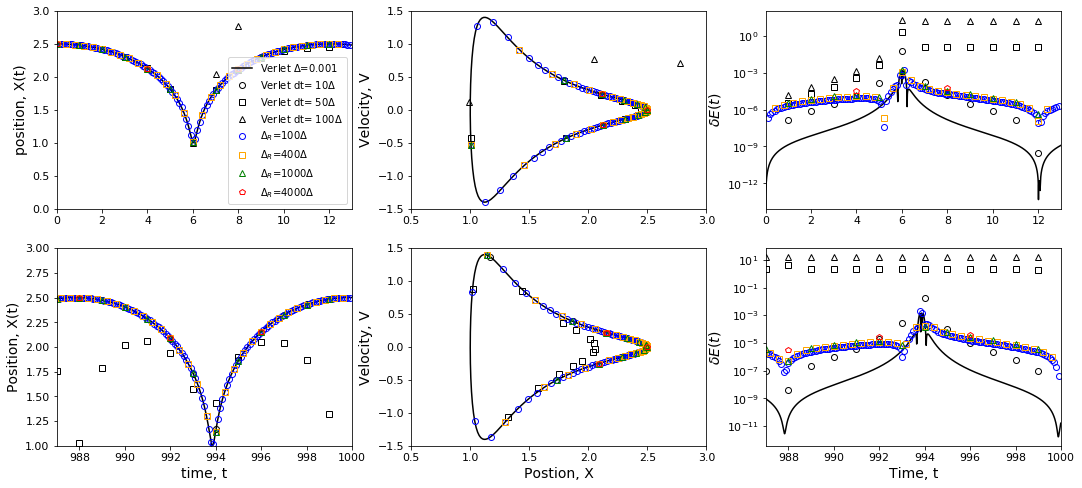
\includegraphics[width=1.0\textwidth]{figures/fig8.png}
%\vspace*{-20pt}
\caption{Dynamics of a particle in a 1D LJ potential ($m=1, x_0=2.5)$ captured by tracking the position $x$ vs. time $t$ (left column), phase space plot of velocity $v$ vs. $x$ (center column), and the deviation in the total energy (right column). Results are shown for the dynamics produced by \V\ and \R. Top row is the dynamics from $t=0$ to $t=13$, and bottom row is the dynamics from $t=987$ to $t=1000$. Black lines are the ground truth results obtained using \V\ with $\Delta=0.001$. Black color circles, squares and triangles represent the results obtained using \V\ with timestep $10\Delta, 50\Delta,$ and $100\Delta$. Blue circles, orange squares, green triangles and red pentagons represent the results obtained using \R\ with $\Delta_{R}=100\Delta, 400\Delta, 1000\Delta,$ and $4000\Delta$ respectively.}
%\vspace*{-15pt}
\label{fig:phasespace}
\end{figure*}

Adam optimizer is used to optimize the error backpropagation. The learning rate of Adam optimizer and the dropout rate in the dropout layer is set to  0.0005 and 0.15 respectively to prevent overfitting. Both learning and dropout rates were selected using a trial-and-error process. The weights in the hidden layers and in the output layer are initialized for better convergence using a Xavier normal distribution at the beginning. Xavier normal distribution is characterized with $0$ mean and $\sigma = 1/(\sqrt{d_i + d_o})$ variance, where $d_i$ and $d_o$ are input and output sizes of the hidden layers, respectively \cite{glorot2010understanding}. The L2 error (mean square loss) between target and predicted trajectories is used for error calculation. LSTM implementation, training, and testing are programmed using scikit-learn, Keras, and TensorFlow ML libraries \cite{chollet2015keras,buitinck2013api,abadi2016tensorflow}. Scikit-learn is used for grid search and scaling, Keras is used to save and load models, and TensorFlow is used to create and train the integrator $\mathscr{R}$. 

\subsection{Additional Experiments and Empirical Results}
\paragraph{Phase diagram for LJ}

This experiment focuses on testing \R\ to predict the time evolution of the 1D LJ system (with particle of mass $m=1$ and initial position $x_0=2.5$). Training dataset comprising of trajectories (positions and velocities) up to $t=200$ simulated using \V\ with \dt$=0.001$ are used to train \R. Figure \ref{fig:phasespace} shows the $1^{\mathrm{st}}$ period (top row) from $t=1$ to $t=13$ and the $75^{\mathrm{th}}$ period (bottom row) from $t=987$ to $t=1000$ of the simulation. The $ 75^{\mathrm{th}}$ period is towards the end of the simulation. For either time periods characterizing the oscillations, the positions predicted by \R\ remain close to the numerically exact result with $\Delta_{\textrm{R}} \in [100\Delta,4000\Delta]$. On the other hand, the trajectory simulated using \V\ shows errors rising with $t$ for timesteps 10\dt, 50\dt, 100\dt\ (all $\le$ \dtR).
Similarly, velocities $v$ produced by \R\ exhibit very small deviations from the ground truth result as evidenced by the phase space plots ($v$ vs. $x$) in Figure \ref{fig:phasespace}. On the other hand, the phase space plot generated using trajectories evolved with \V\ deviated from the ground truth. 
Finally, the total energy produced by \R\ tracks the ground truth result for $t$ up to 1000 and $\Delta_{\textrm{R}} \in [100\Delta,4000\Delta]$, in stark contrast with results using \V\ as the integrator.
\begin{figure*}[htb]
\centering
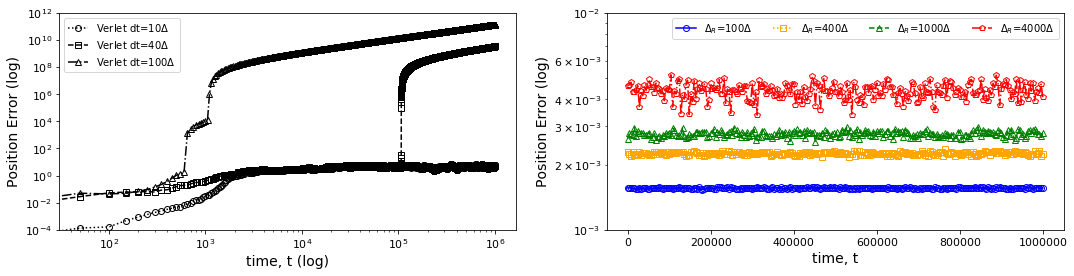
\includegraphics[width=1.0\textwidth]{figures/fig9.png}
%\vspace*{-20pt}
\caption{Average error $\delta r$ (log scale) in position updates (trajectory) vs. time $t$ incurred in a simulation of a $N=16$ particle system with LJ interaction potentials ($\epsilon=2$ and $m=1$) in 3D. Initial positions are randomly selected and velocities are initialized to zero. All results are compared with the ground truth result obtained using \V\ with $\Delta=0.001$. Left plot shows $\delta r$ for the time evolution up to $t=1$ million (log scale) for \V\ using different $dt=10\Delta, 40\Delta, 100\Delta$ values. Right plot shows $\delta r$ for the same time evolution using \R\ with different $\Delta_{R}$=100$\Delta$, 400$\Delta$, 1000$\Delta$, 4000$\Delta$ values. 
}
%\vspace*{-15pt}
\label{fig:manyparticleSI}
\end{figure*}
\paragraph{Many particle experiments}
Figure \ref{fig:manyparticleSI} shows the total error associated with the positions of many particles as a function of time for evolution driven by \R\ and \V. The errors are computed using:
\begin{equation}\label{eq:avg_pos_error}
    \delta r = \frac{1}{N}\sum_{i=1}^{N} \left| \vec{r}_{i, \mathrm{GT}}- \vec{r}_{i, \mathscr{R}}\right|
\end{equation}
where the formula is shown for $\mathscr{R}$. 
The simulated system is $N=16$ particles interacting in 3D with LJ potential under PBC. The ground truth (GT) results for the trajectories are generated using \V\ with $\Delta=0.001$. Note that the training set consisted of dynamics up to $t=2000$ and we intentionally kept the random initial configuration tested here outside the training and testing datasets. 
We find that the trajectory error $\delta r$ associated with the positions predicted by \R\ for \dtR$=100$\dt\ to $4000$\dt\ is $O(10^{-3})$ up to $t=10^6$. On the other hand, $\delta r$ for the system evolved using \V\ with timestep $10\Delta$ increases to $O(10^{-1})$ at around $t \approx 1000$, and $\delta r$ for $40\Delta, 100\Delta$ rises to very large values $>10^{9}$, rendering the time evolution of the system meaningless.

\bibliography{references}

\end{document}
